\documentclass[a4paper]{article}


\usepackage{alphabeta} 
\usepackage{enumitem} 
\usepackage{mathtools}
\usepackage{amsmath, amssymb} 
\usepackage{amsthm}
\usepackage{cancel} 
\usepackage[margin=0.70in]{geometry} 
\geometry{left=2cm,right=2cm,top=2.4cm,bottom=2.4cm}	%the page geometry as defined, A4=210x297mm
\usepackage{graphicx}
\usepackage{wrapfig}
\usepackage[center]{caption}
\usepackage{textcomp}
\usepackage{tabto}
\usepackage{layout}
\usepackage{bm}
\usepackage{minipage-marginpar}
\usepackage[dvipsnames]{xcolor}
\usepackage{hyperref}
\usepackage{dutchcal}
\usepackage{derivative}
\usepackage{esint}
%\usepackage{biblatex}
\usepackage{subcaption}
\usepackage{fancyhdr}
\usepackage{booktabs}\usepackage{derivative}
\usepackage[flushleft]{threeparttable}
\usepackage[capbesideposition=outside,capbesidesep=quad]{floatrow}
\usepackage{derivative}
\usepackage[thinc]{esdiff}
\usepackage{lipsum}
\usepackage{arydshln}
%%RENEW

\newtheorem{problem}{Άσκηση}
\newtheorem*{solution*}{Λύση}
\newtheorem{definition}{Ορισμός}[subsection]
\newtheorem{properties}{Ιδιότητες}[subsection]
\newtheorem{theorem}{Θεώρημα}[subsection]
\newtheorem{protash}{Πρόταση}[subsection]
\newtheorem{porisma}{Πόρισμα}[subsection]
\newtheorem{lemma}{Λήμμα}[subsection]
\newtheorem*{prooof}{Απόδειξη}
\newtheorem*{notes}{Παρατηρήσεις}
\newtheorem*{note}{Παρατήρηση}
\newtheorem*{app}{Εφαρμογή} 
\newtheorem*{example}{Παράδειγμα}
\newtheorem*{examples}{Παραδείγματα}


\newcommand\numberthis{\addtocounter{equation}{1}\tag{\theequation}}
%\renewcommand{\labelenumi}{\roman{enumi}}
\newcommand{\approxtext}[1]{\ensuremath{\stackrel{\text{#1}}{\approx}}}
\renewcommand{\figurename}{Εικόνα.}
\renewcommand{\tablename}{Πίνακας.}
%\renewcommand\refname{New References Header}
\renewcommand*\contentsname{Περιεχόμενα}
%\DeclareDerivative{\odv}{\mathrm{d}}


\title{Απορρόφηση Σωματιδίων β}
\author{Θωμόπουλος Σπυρίδων, ge19042}


\begin{document}
\pagestyle{fancy}
\fancyhead{}
\fancyfoot{}
\fancyhead[LO,LE]{\textbf{03 Απορρόφηση Σωματιδίων β}}
\fancyfoot[CE,CO]{\thepage}

%\begin{titlepage}			%makes a title page. Remember to change the author, CID, username and group number to what is appropriate for you!
%	\centering
%	{\scshape\LARGE Εθνικό Μετσόβιο Πολυτεχνείο\par}
%	{\scshape \LARGE Σ.Ε.Μ.Φ.Ε.\par}
%	\vspace{1cm}
%	{\huge\bfseries Απορρόφηση Σωματιδίων β\par}
%	\vspace{1cm}
%	{\Large\itshape Θωμόπουλος Σπύρος\par}		%remember to change these!
%	
%	%		{\large Group \@group\unskip\strut\par}
%	{\large spyros.thomop@gmail.com/ ge19042@mail.ntua.gr\par \hfill \\}% 		%remember to change these!
%	\vspace{1cm}
%	{\large Ημερμονηνία Παράδοσης 17/05/2022\par}
%\end{titlepage}

\begin{titlepage}




\newcommand{\HRule}{\rule{\linewidth}{0.5mm}}

\includegraphics[width=8cm]{logo1.png}\\[1cm] 
\center 
\quad\\[1.5cm]
\textsl{\Large Εθνικό Μετσόβιο Πολυτεχνείο}\\[0.5cm] 
\textsl{\large Σχολή Εφαρμοσμένων Μαθηματικών και Φυσικών Επιστημών}\\[0.5cm] 
\makeatletter
\HRule \\[0.4cm]
{ \huge \bfseries \@title}\\[0.4cm] 
\HRule \\[1.5cm]
\begin{minipage}{0.4\textwidth}
\begin{flushleft} \large
\emph{Author:}\\
\@author 
\end{flushleft}
\end{minipage}
~
\begin{minipage}{0.4\textwidth}
\begin{flushright} \large

\end{flushright}
\end{minipage}\\[3cm]
\makeatother
%{\large An Assignment submitted for the UoS:}\\[0.5cm]
{\large \emph{Εργαστήριο Πυρηνικής Φυσικής \& Στοιχειωδών Σωματιδίων}}\\[0.5cm]
{\large \today}\\[2cm] 
\vfill 



\end{titlepage}

\subsection*{Σκοπός}
	Ο σκοπός της εν λόγω εργαστηριακής άσκησης είναι ο προσδιορισμός της εμβέλειας των σωματιδίων β με έναν καταμετρητή Geiger-Muller.
\subsection*{Θεωρητικά Στοιχεία}

Στις αρχές του 20ου αιώνα, ο Rutherford κατηγοριοποιήσε τις τότε τρεις γνωστές ακτινοβολίες, α,β και γ, ανάλογα με την διεισδυτικότητά τους. Οι ακτίνες α, δηλαδή πυρήνες Ηλίου, μπορούν να εμποδιστούν από λεπτό φύλλο Αλουμινίου και είναι οι λιγότερο διεισδυτικές. Αντιθέτως, οι ακτίνες γ, δηλαδή φωτόνια υψηλής ενέργειας, είναι οι περισσότερο διεισδυτικές. 
	Οι ακτίνες β, πρόκειται για ηλεκτρόνια ($\beta^-$) ή ποζιτρόνια ($\beta^+$) και η διεισδυτικότητά τους είναι μεταξύ των δύο παραπάνω, της τάξης $\sim cm$ σε Αλουμίνιο. Οι διασπάεις από τις οποίες προκύπτουν είναι οι διασπάσεις β, κατά τις οποίες ένα νετρόνιο μετατρέπεται σε πρωτόνιο και αντίθετα ή πιό συγκεκριμένα, η $\beta^-$ πρόκειται για την $n \rightarrow p + e^- + \overline{\nu_e}$, ενώ η $\beta^+$ για την $p \rightarrow n + e^+ +\nu_e$, η οποία απαιτεί εξωτερικό πεδίο από άλλα νουκλεόνια καθώς το πρωτόνιο έχει χρόνο ημιζωής ~$10^{34}years$, δηλαδή πρακτικά είναι σταθερό.
	
	Ιστορικά, την δεκαετία του 1920, όταν δεν είχαν εισαχθεί στην θεωρία τα νετρίνα, παρατηρήθηκε ότι ενέργεια του σωματιδίου β κατα την διάσπαση αυτή δεν ήταν σταθερή, αλλά εμφανιζοταν ένα φάσμα. Χανόταν δηλαδή ένα ποσό ενέργειας και ως εκτούτου παραβιαζονταν μία θεμελιώδης αρχή της φυσικής. Κάποιοι φυσικοι της εποχής, όπως ο Bohr εξέτασαν την πιθανότητα εγκατάληψης του εν λόγω αξιώματος στον μικρόκοσμο, ενώ άλλοι δεν ήταν πρόθυμοι για κάτι τέτοιο και το 1932 προτάθηκε από τον Pauli η ύπαρξη ενός σωματιδίου που θα ισοστάθμιζε το ποσό ενέργειας που φαινόταν να χάνεται.
	
	
	Ο τρόπος που μπορούμε να ανιχνεύσουμε το συνεχές φάσμα των ηλεκτρινίων β είναι μέσω του τρόπου με τον οποίο αλληλεπιδρούν με κάποιο υλικό. Συγκεκριμένα, τα ηλεκτρόνια χαμηλής ενέργειας συγκρούονται ανελαστικά (με δυναμικό Coulomb) με τα ηλεκτρόνια των ατόμων του υλικού που διασχίζουν, προκαλώνας διέγερση και ιονισμό. Έτσι χάνουν ενέργεια ως αποτέλεσμα πολλών συγκρούσεων μικρής απώλειας (αφού για ιονισμό ή διέγερση των ατομικών e απαιτείται ενέργεια $\sim eV$) ακολουθώντας την καμπύλη Bethe-Bloch. Αντιθέτως, αν τα σωμάτια β είναι υψηλής ενέργειας, ο κυρίαρχος μηχανισμός απωλειών είναι μέσω της ακτινοβολίας πέδησης, η οποία είναι μεγαλύτερη για μεγάλη επιτάχυνση και για μικρή μάζα $$E_{Brem}/E_0 \sim |\vec{a}|^2 \sim Z^2/m^2$$. 
	
	Ο λόγος των δύο απωλειών ανά μονάδα μήκους είναι 
		\begin{equation}\label{eq1}
			\frac{(dE/dx)_{Brem}}{(dE/dx)_{BB}} = \frac{EZ}{800}
		\end{equation}

Οι δύο παραπάνω μηχανισμοί απώλειας ενεργειας θα οδηγήσουν τα σωματίδια β να χάσουν όλη τους την ενέργεια, δηλαδή να σταματήσουν και έπειτα να απορροφηθούν απ' το υλικό. Το μήκος που έχουν διανύσει εντός του υλικού εως ότου σταματήσουν ονομάζεται \textit{εμβέλεια}. 
Έστω ότι θέλω να βρώ την μείωση της ροής (\#σωματιδίων που διασχίζουν επιφάνεια κάθετη την δέσμη /$m^2s$) μίας δέσμης σωματιδίων β που διασχίζει ένα υλικό σαν συνάρτηση του πάχους μάζας του (ανηγμένη απόσταση που διανύει εντός που υλικού προς την πυκνότητά του, δηλαδή $ x=\rho \cdot t)$ [$mgr/cm^2$]). 
Τότε, για μεταβολή της απόστασης κατά dt, το πάχος μάζας μεταβάλλεται κατα dx και η ροή μειώνεται ως εξής 
	\begin{align*}
		\frac{d\Phi}{\Phi} \propto -dx\Rightarrow\frac{d\Phi}{\Phi}= - \mu dx \Rightarrow \int d\Phi/\Phi = - \int \mu dx \Rightarrow
			\Phi = \Phi_0 exp(-\mu x)
	\end{align*}	  
	όπου μ είναι η σταθερά αναλογίας για την εν λόγω απώλεια ή αλλιώς ο συντελεστής απορρόφησης. Όμως, επειδή $\Phi \propto N$, όπου Ν ο αριθμός των σωματιδίων, θα έχουμε 
	\begin{equation}\label{eq2}
		N = N_0 exp(-\mu x)
	\end{equation}
Από την παραπάνω σχέση θα δίνεται επίσης και ο αριθμός των σωματιδίων που καταγράφει ένας καταμετρητής Geiger-Muller σαν αυτόν που χρησιμποιούμε στην άσκηση. Η μορφή της καμπύλης (\ref{eq2}) είναι εμπειρικός νόμος και χαρακτηρίζει κυρίως τα σωματίδια β χαμηλής ενέργειας.

	
	Αν θέλουμε να υπολογίσουμε την μέγιστη ενέργεια κάποιων ηλεκτρονίων που προέρχονται π.χ. από μία ραδιενεργό πηγή, τότε δεν μπορούμε να την μετρήσουμε άμεσα, αλλά θα πρέπει να την συνδέσουμε με κάποιο άλλο μέγεθος που είναι πειραματικά μετρήσιμο. Αυτό το μέγεθος είναι η εμβέλεια η οποία μπορεί να προσδιοριστεί αυξάνοντας διαδοχικά το πάχος ενός στόχου και καταμετρώντας τα σωματίδια που διέρχονται. Το πάχος στο οποίο σταματάει η διέλευση των ηλεκτρονίων από την πηγή είναι αυτό το οποίο θεωρούμε ως την εμβέλειά τους στο εκάστοτε υλικό την οποία στη συνέχεια την ανάγουμε στο πάχος μάζας για να μπορούμε να γενικεύσουμε για όλα τα υλικά. Η σχέση που συνδέει μέγιστη ενέργεια και εμβέλεια είναι 
	\begin{align}\label{eq3}
			R = 0.11 (\sqrt{1+22.4E_{max}^2} - 1) , \text{ όπου $[E_{max}]=MeV$}
	\end{align}
	
	Υπάρχει ένα πρόβλημα στον υπολογισμό της εμβέλειας των ηλεκτρονίων. Καθώς αυτά εκπέμπονται από την πηγή, κατά την κίνησή τους στο υλικό θα εκπέμπονται ταυτόχρονα και ακτίνες γ, σκληρή συνιστώσα. 
	Αυτά τα νέα φωτόνια γ, κατά την αλληλεπίδρασή τους με την ύλη, δίνουν όλη (ή σχεδόν όλη) την ενέργειά τους σε νέα ηλεκτρόνια που προέρχονται από το υλικό μέσω του μηχανισμού του φωτοηλεκτρικού φαινομένου ή στα ήδη υπάρχοντα απο τις ακτίνες β, μέσω της σκέδασης Compton. Έτσι ενδέχεται να δημιουργηθούν νέα ηλεκτρόνια τα οποία αδυνατούμε να ξεχωρίσουμε από όσα προέρχονται πράγματι από την διάσπαση β. Όπως θα δούμε στην περίπτωση του $^{90}Sr$ η συνεισφορά των ακτίνων γ, που αλλιώς καλείται σκληρή συνιστώσα είναι αμελητέα.
	
	
\subsection*{Πειραματική Διάταξη}
	 Η πειραματική διάταξη αποτελείται από: 
	 	\begin{itemize}
	 		\item[.] Απαριθμητή Geiger-Muller
	 		\item[.] Μονάδα επικονωνίας με τον G-M
	 		\item[.] $^{90}_{38}Sr$ ως πηγή σωματιδίων β
	 		\item[.] Απορροφητή Αλουμινίου
	 	\end{itemize}
	 	
\subsubsection*{Λειτουργία του Geiger-Muller}
	
	Ο καταμετρητής Geiger-Muller πρόκειται για έναν ανιχνευτή αερίου που χρησιμεύει για την καταμέτρηση φορτισμένων σωματιδίων. Γεωμετρικά, είναι ένας κοίλος κύλινδρος στο κέντρο του οποίο έχουμε τοποθετήσει ένα λεπτό ηλεκτρόδιο. Εφαρμόζοντας μία διαφορά δυναμικού μεταξύ κελύφους-ηλεκτροδίου, δημιουργούμε ηλεκτρικό πεδίο στο εσωτερικό του ανιχνευτή το οποίο θα οδηγεί τα φορτισμένα σωματίδια που εισέρχονται σε αυτόν προς τους δύο πόλους του. Επομένως θα δημιουργείται ένα ηλεκτρικό σήμα το οποίο και θα ανιχνεύουμε. Όμως, αν ο εσωτερικός χώρος του ανιχνευτή ήταν κενός, ενδεχομένως η επίδραση του πεδίου στα πολύ ενεργητικά σωματίδια να ήταν ανεπαίσθητη και όσα κατέληγαν στους πόλους θα ήταν πολύ λίγα για να παράξουν ένα ανιχνεύσιμο σήμα. Άρα θα πρέπει με κάποιον τρόπο να ενισχύσουμε τον αριθμό των φορτισμένων σωματιδίων που καταλήγουν στους πόλους. 
	
	Η εν λόγω ενίσχυση επιτυγχάνεται με την εισαγωγή ενός αερίου στο εσωτερικό του ανιχνευτή μας (Ar, $H_2$ για ανίχνευση ακτινοβολίας β).
	 Τώρα, όταν εισέρχεται ένα σωματίδιο, στην περίπτωσή μας ηλεκτρόνιο, ενδέχεται να αλληλεπιδράσει με κάποιο από τα άτομα/μόρια του αερίου ιονίζοντάς το και παράγοντας ένα ζεύγος ιόντος-ηλεκτρονίου. Αυτά τα ηλεκτρόνια καλούνται Primary Ionization Electrons (PIE). Πλέον έχουμε δύο ελεύθερα ηλεκτρόνια τα οποία επιταχύνονται προς την άνοδο (υψηλότερο δυναμικό) χάρη στο πεδίο που έχουμε δημιουργήσει στο εσωτερικό. Αν το πεδίο είναι αρκούντως ισχυρό, τα ηλεκτρόνια ενδεχομένως ιονίσουν και άλλα άτομα/μόρια του αερίου αυξάνοντας έτσι σταδιακά τον αριθμό των ηλεκτρονίων που θα φτάσουν στην άνοδο και θα ανιχνευτούν ως σήμα. Ο λόγος των ηλεκτρονίων που φτάνουν στην άνοοδο προς τα PIE ονομάζεται παράγοντας πολλαπλασιασμού $M=N/N_0=exp(ax) < 10^6$ και αυξάνεται εκθετικά με το πάχος του αερίου. Αυτό το φαινόμενο κατά το οποίο ένα αρχικό ηλεκτρόνιο δημιουργεί έναν καταιγισμό ηλεκτρονίων ονομάζεται \textit{φαινόμενο της χιονοστιβάδας.}
	
	Στην πραγματικότητα όλα τα παραπάνω φαινόμενα είναι στατιστικής φύσεως. Δηλαδή, τα PIE έχουν μία πιθανότητα να αλληλεπιδράσουν με τα άτομα/μόρια του αερίου και στην συνέχεια το ηλεκτρικό πεδίο δεν τα επιταχύνει προς μία κατεύθυνση μεμονωμένα ηλεκτρόνια, αλλά προσανατολίζει την θερμική κίνηση όλων των ηλεκτρονίων (αν $\vec{Ε}=0$, τότε $<u_{therm}> =0$) προς την κατεύθυνση της ανόδου.
	
	Επίσης, η λειτουργία του ανιχνευτή μπαίνει σε διαφορετικές περιοχές ανάλογα με την διαφορά δυναμικού μεταξύ των δύο ηλεκτροδίων. Ενεδεικτικά, όταν είναι πολύ χαμηλή, τα ηλεκτρόνια που απομακρύνονται από τα άτομα δεν προλαβαίνουν να επιταχυνθούν επαρκώς, επανασυνδέονται με τα θετικά ιόντα και έτσι έχουμε πολύ ασθενές σήμα. Αν αυξήσουμε την διαφορά δυναμικού (αφού προσπεράσουμε κάποιες περιοχές), μπαίνουμε στην αναλογική περιοχή, στην οποία η κάθε χιονοστιβάδα που δημιουργείται είναι ανεξάρτητη από τις υπόλοιπες και ως εκτούτου, οι τελικές ανιχνεύσιμες χιονοστιβάδες είναι ανάλογες με τον αριθμό των PIE. Η περεταίρω αύξησή της (πάλι παραλείπονται περιοχές), μας οδηγεί στην περιοχή Geiger η οποία χαρακτηρίζεται από την ανεξαρτησία των τελικών ανιχνεύσιμων γεγονότων από τον αρχικό ιοντισμό (Geiger Discharge). 
	Εδώ εμφανίζονται πιό ενισχυμένες χιονοστιβάδες οι οποίες μπορούν να παράξουν νέες. Σε κάποια κρίσιμη τιμή της διαφοράς δυναμικού, η κάθε μία χιονοστιβάδα παράγει κατά μέσο όρο $\geq 1$ νέες, άρα έχουμε εκθετική άυξηση των συνολικών χιονοστιβάδων που ανιχνεύονται και ο τελικός παλμός είναι της τάξης των Volt. 
	Η δημιουργία μίας νέας χιονοστιβάδας από μία αρχική, γίνεται μέσω εκπεμπόμενων φωτονίων. Καθώς ένα αρκετά ενεργητικό ηλεκτρόνιο ιονίζει ένα άτομο/μόριο, δημιουργείται ένα κενό σε κάποιον από τους εσωτερικούς φλοιούς. 
	Όταν γίνει μία μετάπτωση προς αυτή την κενή θέση εκπέμπεται φωτόνιο το οποίο δύναται να δημιουργήσει ελεύθερα ηλεκτρόνια, μακριά από την αρχική χιονοστιβάδα, είτε αλληλεπιδρώντας με τα ασθενώς δεσμευμένα ατομικά/μοριακά ηλεκτρόνια είτε μέσω φωτοηλεκτρικού φαινομένου με το μέταλλο της ανόδου.
	
	Καθώς τα ηλεκτρόνια κινούνται προς την άνοδο, τα ιόντα, έχοντας πολυ μεγαλύτερη μάζα, δεν προλαβαίνουν να μετακινηθούν προς την κάθοδο και υπάρχει ένα νέφος θετικών φορτίων γύρω της ανόδου που μειώνει το ηλετρκικό πεδίο και επιδεινώνει το ιονισμό. Όμως όταν ο κύκλος μίας χιονοστιβάδας ολοκληρωθεί, θα πρέπει τα ιόντα να έχουν επιστρέψει στην κάθοδο. Κατά την επιστροφή τους ενδεχομένως κάποια να έχουν αρκετά υψηλή ενέργεια ($E_{ion} > 2\cdot$(Ενέργεια για απομάκρυνση 1e από την κάθοδο))  ώστε να απελευθερώσουν ηλεκτρόνια τα οποία με την σειρά τους θα δημιουργήσουν νέες χιονοστιβάδες oι οποίες όμως δεν οφείλονται στο σωματίδιο που θέλουμε να ανιχνεύσουμε δημιουργώντας έτσι έναν ανεπιθύμητο παλμό που ενδεχωμένως να καταστρέψει και τον ανιχνευτή μας. Γι' αυτό, είναι αναγκαίο να εισάγουμε ένα δεύτερο αέριο το οποίο θα επιβραδύνει τα ιόντα και θα περιορίζει αυτούς τους ανεπιθύμητους ιονισμούς, το \textit{αέριο απόσβεσης}.
	
	Ένα αρνητικό στοιχείο των καταμετρητών G-Μ είναι ο μεγάλος Ανενεργός Χρόνος, δηλαδή ο χρόνος που μεσολαβεί από την επεξεργασία ενός συμβάντος εώς την στιγμή όπου ο ανιχνευτής θα είναι σε θέση να ανιχνεύσει ένα νέο. 
	Κατά την επιστροφή των ιόντων στην κάθοδο, μεταβάλλεται το ηλεκτρικό πεδίο με τρόπο τέτοιον ώστε να θωρακίζει την έλξη των ηλεκτρονίων από την άνοδο και οι νέες χιονοστιβάδες να μην είναι τόσο ισχυρές. % καθώς τα θετικά ιόντα θα επιβραδύνουν νέα ηλεκτρόνια που κινούνται προς την άνοδο 
	Κατ' επέκταση ο χρόνος αυτός θεωρείται νεκρός για τον ανιχνευτή, δηλαδή όλα τα γεγονότα που συμβαίνουν τότε δεν θα μπορούν να ανιχνευτούν. Εν γένει αυτός ο χρόνος είναι της τάξης των $50-100\mu s$.
 		
 		\subsubsection*{Ιδιότητες Πηγής $^{90}Sr$}
 		
 		
	Η ενεργότητα της πηγής όταν κατασκευάστηκε ήταν $R_0=0.1\mu Ci$, ο χρόνος ημιζωής είναι $t_{1/2}=28.8yr$, άρα $\lambda=ln(2)/t_{1/2} =0.024y^{-1}$. Συνεπώς, σύμφωνα με τον νόμο των ραδιενεργών διασπάσεων $R = R_0 exp(-\lambda t)$, όπου t σε years και δεδομένου ότι κατασκευάστηκε 07/2003, η ενεργότητά της όταν πραγματοποιήθηκε η άσκηση ήταν $R =R_0exp(-0.024\cdot 19.25) =  0.63R_0 = 0.063\mu Ci\simeq2300 διασπασεις/sec \simeq 1.4\times10^5 διασπασεις/min$.
	Θα επανέλθω σε αυτό το ζήτημα στο τελευταίο ερώτημα για να δικαιολογήσω πως αυτή τη συλλογιστική είναι λάθος.	
	
%	Μέχρι στιγμής έχουμε λάβει υπόψιν μόνο την διάσπαση του $^{90}Sr$. 
	
	\subsubsection*{Ιδιότητες ανιχνευτή}
	Δεδομένου ότι η πηγή απέχει $d=(5.2\pm 0.1) cm$ από τον ανιχνευτή και ότι η ακτίνα της είναι $\rho = (1.4\pm 0.1)cm$, μπορούμε να υπολογίσουμε την στερεά γωνία την οποία καλύπτει ο ανιχνευτής μας θεωρώντας την πηγή σημειακή και πως εκπέμπει ισότροπα σε όλον τον χώρο: 
		\begin{align*}
			d\Omega =& sin\theta d\theta d\phi \Rightarrow\\
			\Omega  =& \int_0^a  sin\theta d\theta \int_0^{2\pi} d\phi \Rightarrow\\
			        =& 2\pi (1-cos\alpha) \Rightarrow\\
			        =& 2\pi \left(1-\frac{d}{\sqrt{d^2+\rho^2}}\right)
		\end{align*}		 
 		Άρα \footnotemark
 		\vspace{-0.7cm}
 		\begin{align*}\label{eq4}
 			\Omega = (0.22 \pm 0.05) ster 	\numberthis
		\end{align*} 	
	\footnotetext{Το σφάλμα προκύπτει από διάδοση $\delta\Omega= \sqrt{\left( \pdv{\Omega}{R}\delta R\right)^2 + \left( \pdv{\Omega}{d}\delta d\right)^2} =\sqrt{\left( \frac{Rd}{(R^2+d^2)^{3/2}} \right)^2 + \left( \frac{R^2}{(R^2+d^2)^{3/2}}\right)^2}=0.0483$}	 		
\subsection*{Πειραματική Διαδικασία - Επεξεργασία Μετρήσεων}

	Μετράμε αρχικά την ακτινοβολία υποβάθρου, δηλαδή όλα τα γεγονότα $K_{back}$ που δεν προέρχονται από την ραδιενεργό πηγή μας, για 6min. 
	Έπειτα, τοποθετούμε την πηγή, μετράμε επίσης τα γεγονότα $K_\beta$ για 3min και διαδοχικά προσθέτουμε φύλλα Αλουμινίου. Με κάθε προσθήκη μετράμε πάλι τα γεγονότα στον καταμετρητή μας για 3min. Όταν τα γεγονότα γίνουν ίσα με τα γεγονότα υποβάθρου, τότε θεωρούμε πως έχουμε βρει την εμβέλεια των ηλεκτρονίων της πηγής μας και σταματάμε τις μετρήσεις.
	Ανάγουμε τα καταγεγραμμένα γεγονότα σε ρυθμό, δηλαδή γεγονότα/min, $N_{back}$ και $N_{\beta}$ αντίστοιχα για το υπόβραθρο και την ακτινοβολία β. Τα αποτελέσματα φαίνονται στον Πίνακα 1. 
		\begin{table}[h!]
			\centering
			\begin{tabular}{|*6r|}
				Φύλλα Al & $x_{Al}(mg/cm^2)$ & $K_\beta$ & $N_\beta (min^{-1})$ & $N_\beta - N_{back} (min^{-1})$ & $\delta(N_\beta-N_{back})$\footnotemark\\ 
				\midrule
				\multicolumn{6}{c}{\textbf{Background}}\\
				\midrule 
				- & - & 112 & 19 & - & 3 \\ 
				\midrule
				\multicolumn{6}{c}{\textbf{Beta Rays}}\\
				\midrule
				0&0&8152&2717&2698&17\\
1&110&5630&1877&1858&14\\
2&220&3779&1260&1241&12\\
3&330&2183&728&709&9\\
4&440&1192&397&378&7\\
5&550&608&203&184&5\\
6&710&198&66&47&2\\
7&870&81&27&8&1\\
8&1030&65&22&3&1\\
9&1190&50&17&-2&1
%	0&0&8152&2717&2699&30.1\\
%1&110&5630&1877&1858&25.0\\
%2&220&3779&1260&1241&20.5\\
%3&330&2183&728&709&15.6\\
%4&440&1192&397&379&11.5\\
%5&550&608&203&184&8.2\\
%6&710&198&66&47&4.7\\
%7&870&81&27&8&3.0\\
%8&1030&65&22&3&2.7\\
%9&1190&50&17&-2&2.4
			%\midrule
			\end{tabular}
		\caption{ Πειραματικά Δεδομένα}
		\end{table}
		
		\footnotetext{$\delta(N_\beta-N_{back})=\sqrt{N_\beta-N_{back}}/mins$ }
		
		Από τα παραπάνω πειραματικά δεδομένα μπορούμε να φτιάξουμε την καμπύλη $ln(N_\beta-N_{b}) = f(x_{Al})$ η οποία είναι μία ευθεία και προκύπτει από την μέθοδο ελαχίστων τετραγώνων. Το σφάλμα στον y άξονα προκύπτει από την σχέση $\delta(ln(N)) = \delta(N) /N = \sqrt{K}/(N*mins) = \delta(N) /N = \sqrt{K}/(N*3)$. Η γραφική παράσταση φαίνεται στην Εικόνα 1. Επίσης σχεδιάζω την ευθεία υποβάθρου $y_b = ln(N_b)=ln(19)$
		, η οποία έχει  σφάλμα $\delta y_b = \delta N_b/N_b = 0.1/19=0.01$. Από την γραφική παράσταση έχουν αποκλειστεί τα 4 τελευταία σημεία. Αυτό διότι η αβεβαιότητα που έχουμε κοντά στο υπόβαθρο είναι μεγάλη.
		\begin{figure}[h!]
			\centering
			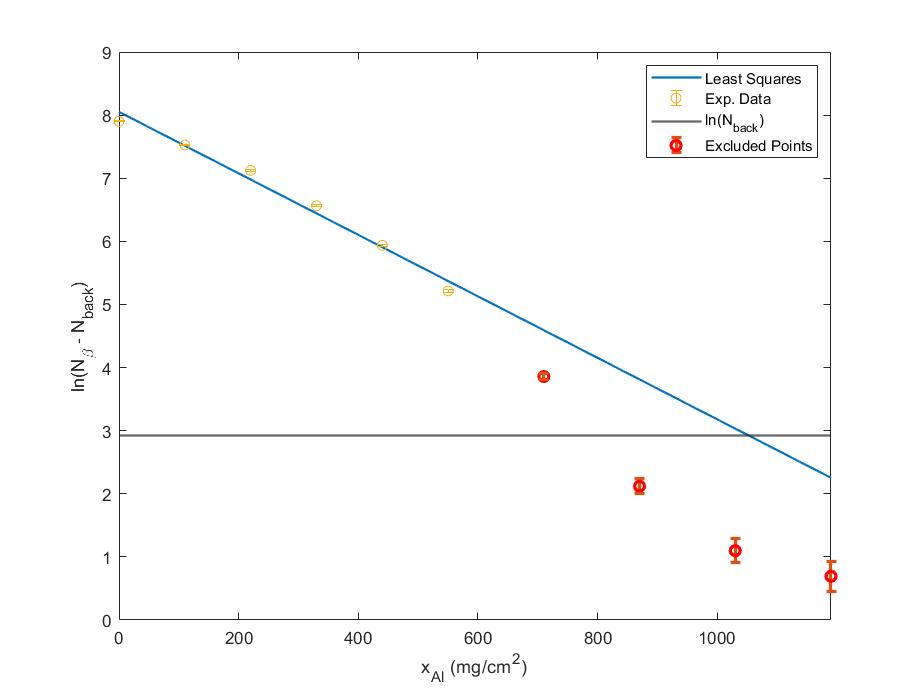
\includegraphics[scale=0.4]{fitt1_excl}
			\caption{$ln(N_\beta-N_b) - x_{Al}$}
		\end{figure}
		
		
		Η ευθεία που προκύπτει είναι η 
			\begin{align*}
				ln(N_\beta - N_b) =& A \cdot x_{Al} + B \\
				A                 =& (-4.9\pm0.8)10^{-3}, [cm^2/mg]\\ 
				B                 =& (8.1\pm0.3)
			\end{align*}

%Επίσης, το σημείο τομής της με την ευθεία υποβάθρου $y =ln(N_b)$, είναι το 
%	\begin{align*}
%		(R, y ) = (825, 2.9 ) 
%	\end{align*}
		Συνεπώς η εμβέλεια των σωματιδίων β στο Αλουμίνιο, από την σχέση  $y_R = y_b\Rightarrow A\cdot R+ B = y_b\Rightarrow R = (y_b-B)/A$, είναι\footnotemark
			\begin{align*}
				R = (1055 \pm 182) mg/cm^2
			\end{align*}
			
			\footnotetext{%Το σημείο προκύπτει ως εξής $y_R = y_b\Rightarrow A\cdot R+ B = y_b\Rightarrow R = (y_b-B)/A = 817mg/cm^2$ \\ 
				Το σφάλμα προκύπτει από διάδοση $\delta R=\sqrt{\left(\pdv{R}{A}\delta A\right)^2 + \left(\pdv{R}{B}\delta B\right)^2 + \left(\pdv{R}{y_b}\delta y_b \right)^2} = \sqrt{\left( \frac{B-y_b}{A^2} \delta A\right)^2 + \left(  \frac{1}{A}\delta B\right)^2+ \left( \frac{1}{A} \delta y_b \right)^2} = 57$}
				
				Από την σχέση (\ref{eq3}) παίρνω την μέγιστη ενέργεια των εισερχομένων σωματιδίων β και το αντίστοιχο σφάλμα τους \footnotemark
				\begin{align*}
					E_{max} = (2.2 \pm 0.4) MeV
				\end{align*}
				
				\footnotetext{Έχουμε $E_{max} = \sqrt{\left( (R/0.11+1)^2 -1)/22.4\right)}\simeq 1.784 \simeq 1.8MeV$ και από διάδοση παίρνουμε $\delta E_{max} = \pdv{E_{max}}{R} \delta R = \frac{R/0.11 + 1 }{E_{max} 0.11 \cdot 22.4}\delta R=0.0.3536 MeV \simeq 0.4 MeV $}
				
				\textcolor{red}{ΕΡΩΤΗΜΑ 5 }Μέχρι αυτό το σημείο έχουμε αγνοήσει την ύπαρξη της σκληρής συνιστώσας (ακτίνες γ που παράγονται από την αλληλεπίδραση των σωματιδίων-β της πηγής με το υλικό του απορροφητή)
				%εκπέμπονται από την πηγή), 
				,θεωρώντας την αμελητέα. Τώρα, θα επιβεβαιώσουμε αυτήν την υπόθεση. Από την σχέση (\ref{eq1}) βρίσκουμε τον λόγο απωλειών των ηλεκτρονίων λόγω ακτινοβολίας και λόγω αλληλεπίδρασης με το αέριο.
				\begin{align*}
					\frac{(dE/dx)_{Brem}}{(dE/dx)_{BB}} = \frac{EZ}{800} = \frac{1.6\times10^{-3} \cdot 17}{800} = 3.4\times10^{-5}
				\end{align*}			
			Άρα μπορούμε να θεωρήσουμε αμελητέες τις απώλειες ενέργειας των ηλεκτρονίων από εκπομπή ακτινοβολίας όπως έχουμε κάνει σε όλη την ανάλυση. 
			
			
			\textcolor{red}{ΕΡΩΤΗΜΑ 6} Με βάση το λογισμικό ESTAR, η εμβέλεια των σωματιδίων β με ενέργεια περίπου ίση με την μέγιστη ενέργεια των σωματιδίων του πειράματός μας, δηλαδή $E_1=2.0MeV$, θα είναι $R_{1,STAR} = 1244 mg/cm^2$.
			Η πειραματική τιμή είναι $R=1055 mg/cm^2$ και έχει απόκλιση από την θεωρτηική $\delta R \simeq 15\% $ η οποία είναι σημαντική. Αυτό ενδεχομένως να οφείλεται στο ότι ο προσδιορισμός του υποβάθρου, επομένως και του σημείου όπου σταματάμε τις μετρήσεις, έχει μεγάλο στατιστικό σφάλμα.
			
		\textcolor{red}{ΕΡΩΤΗΜΑ 7} Γνωρίζουμε πως η ενεργότητα που αναγράφεται στην πηγή την στιγμή του πειράματος ήταν $R=0.063\mu Ci = 1.4\times10^5διασπασεις/min$, τις οποίες θα ανιχνεύαμε αν καλύπταμε στερεά γωνία $4\pi$ με έναν ιδανικό ανιχνευτή.
		%. Δεδομένου ότι $1\mu Ci = 0.37\times 10^5$ διασπάσεις/s, περιμένουμε πως στην πηγή μας θα γίνονται $R=0.023\times10^5 = 2300$διασπάσεις/s, άρα σε συνολικό χρόνο ενός λεπτού, περιμένουμε $N_3= R\cdot1min = R\cdot60sec \simeq138\times10^3$ διασπάσεις τις οποίες θεωρητικά θα ανιχνεύαμε αν καλύπταμε στερεά γωνία $4\pi$ με έναν ιδανικό ανιχνευτή.
		 Όμως επειδή κανένα από αυτά τα δύο δεν είναι δυνατό, μπορούμε να κάνουμε μία αναγωγή στην στερεά γωνία που καλύπτει ο καταμετρητής μας η οποία προκύπτει από την σχέση (\ref{eq4}), $\Omega = (0.22 \pm 0.05) ster$. Θεωρούμε πως η εκπομπή γίνεται ισότροπα προς όλον τον χώρο και πως στην στερεά γωνία του καταμετρητή μας εκπέμπονται $N_\Omega$ σωματίδια ανά λεπτό. Τότε έχουμε ότι 
	
		\begin{align*}\label{eq5}
			N_\Omega = \frac{R\cdot \Omega}{4\pi} = \frac{1.4\times10^5\cdot 0.22}{4\pi}\simeq 2400 \numberthis
		\end{align*}		
		ωστόσο, εμείς ανιχνεύσαμε $\simeq2700$ διασπάσεις ανά λεπτό. Άρα ο συντελεστής απόδοσης είναι 
			\begin{align*}
				M = \frac{N_{exper} }{N_\Omega} = \frac{2700}{2400} > 1 
			\end{align*}
			
		Προφανώς το παραπάνω συμπέρασμα, ότι δηλαδή ανιχνεύουμε περισσότερα γεγονότα από τις διασπάσεις είναι εξωφρενικό ( αυτός ήταν ο λόγος για τον οποίο καθυστέρησε τόσο η παράδοση της αναφοράς). Μέχρι στιγμής δεν έχουμε λάβει υπόψιν καθόλου τις διασπάσεις του Υτρίου.
		
		Έστω ότι $N_1: Sr \& N_2:Y$ τότε έχουμε την παρακάτω διαδικασία εντός της πηγής \textit{$N_1\rightarrow N_2 \rightarrow  Zr$}.
		Άρα έχουμε πως η μόνη συνεισφορά στην αλλαγή του πληθυσμού του $N_1$ προέρχεται από την διάσπασή του σε Υ, συνεπώς από νόμο ραδιενεργών διασπάσεων έχουμε ότι 
		\begin{align*}
			dN_1 =& -\lambda_1 N_1dt \Rightarrow\\
			N_1  =& N_0 e^{-\lambda t} \numberthis
		\end{align*}
	Ακόμη, η αλλαγή του πληθυσμού των Υ προέρχεται τόσο από την ραδιενεργό διάσπασή του όσο και από την διάσπαση του Sr σε Υ, άρα 
	\begin{align*}
		d N_2 =& \underbrace{-\lambda_2 N_2 dt}_{Ραδιενεργ.} + \underbrace{\lambda_1 N_1 dt}_{Διάσπ. Sr} \Rightarrow \\ 
		 \dot{N_2} + \lambda_2 N_2 = &\lambda_1 N_{0}e^{-\lambda_1 t}   
	\end{align*}
	Η λύση είναι το άθροισμα της λύσης της ομογενούς και της ειδικής λύσης που επιλύει την μη ομογενή.
	
	Η λύση της ομογενούς, $\dot{N_2} + \lambda_2N_2=0$, είναι $N_{2,hom} = A e^{-\lambda_2t}$. Η μη ομογενής επιδέχεται μία εκθετική λύση της μορφής $Be^{-\lambda_1t}$. Αντικαθιστώντας παίρνουμε: 
	\begin{align*}		
		-\lambda_1 B e^{-\lambda_1t} +\lambda_2 B e^{-\lambda_1 t} =& \lambda_1N_{0}e^{-\lambda_1t}\Rightarrow\\
		-\lambda_1B+\lambda_2B =& \lambda_1N_{0} \Rightarrow\\ 
		B(-\lambda_1+\lambda_2) = & \lambda_1N_{0} \Rightarrow\\ 
		B =&\frac{\lambda_1N_{0}}{\lambda_2-\lambda_1}
	\end{align*}

Άρα η λύση της εξίσωσης είναι 
	\begin{align*}
		N_2(t) = Ae^{-\lambda_2t} + \frac{\lambda_1 N_0}{\lambda_2-\lambda_1}e^{-\lambda_1t} 
	\end{align*}
	Την χρονική στιγμής $t=0$ δεν υπήρχαν πυρήνες Υ, άρα $N_2(t=0) =0$ και γι' αυτό η σταθερά είναι ίση με $A = -B$. Άρα η συνολική λύση είναι 
	\begin{align*}
		N_2(t) =& \frac{\lambda_1 N_0}{\lambda_2-\lambda_1} (e^{-\lambda_1t} - e^{-\lambda_2t}) \xRightarrow{\tau_{1/2, 1}>>\tau_{1/2, 2}\Rightarrow \lambda_1<<\lambda_2} \\
		N_2(t) =& \frac{\lambda_1 N_0}{\lambda_2-\lambda_1} ( 1 - e^{-\lambda_2t})  \numberthis
	\end{align*}
	
	Τώρα η συνεισφορά των πυρήνων $N_2$ στην ενεργότητα είναι 
		\begin{align*}
			R_2 =& \lambda_2 N_2  \Rightarrow\\
		    R_2 =& \frac{\lambda_1\lambda_2}{\lambda_2-\lambda_1}N_0(1-e^{-\lambda_2t}) \Rightarrow\\
		    =& \lambda_1 \frac{1}{1-\lambda_1/\lambda_2}N_0 (1-e^{-\lambda_2t})\xRightarrow{\lambda_1<<\lambda_2} \\
		    =& \lambda_1(1-\frac{\lambda_1}{\lambda_2})N_0 (1-e^{-\lambda_2t})\xRightarrow{1st order to \lambda_1} \\ 
		    =& \lambda_1N_0(1-e^{-\lambda_2t})\numberthis 
	\end{align*}			
	
	και προφανώς $R_1(t) = \lambda_1 N_1=\lambda_1 N_0 e^{-\lambda_1t}$. 
	Παρακάτω φαίνεται μία γραφική παράσταση (Eικόνα (\ref{fig2}))  των παραπάνω σχέσεων $R_1(t), R_2(t), R(t)=R_1(t)+R_2(t)$ για την περίπτωσή μας, όπου $\lambda_2<<\lambda_1$.
	
	\begin{figure}[h!]
		\centering
		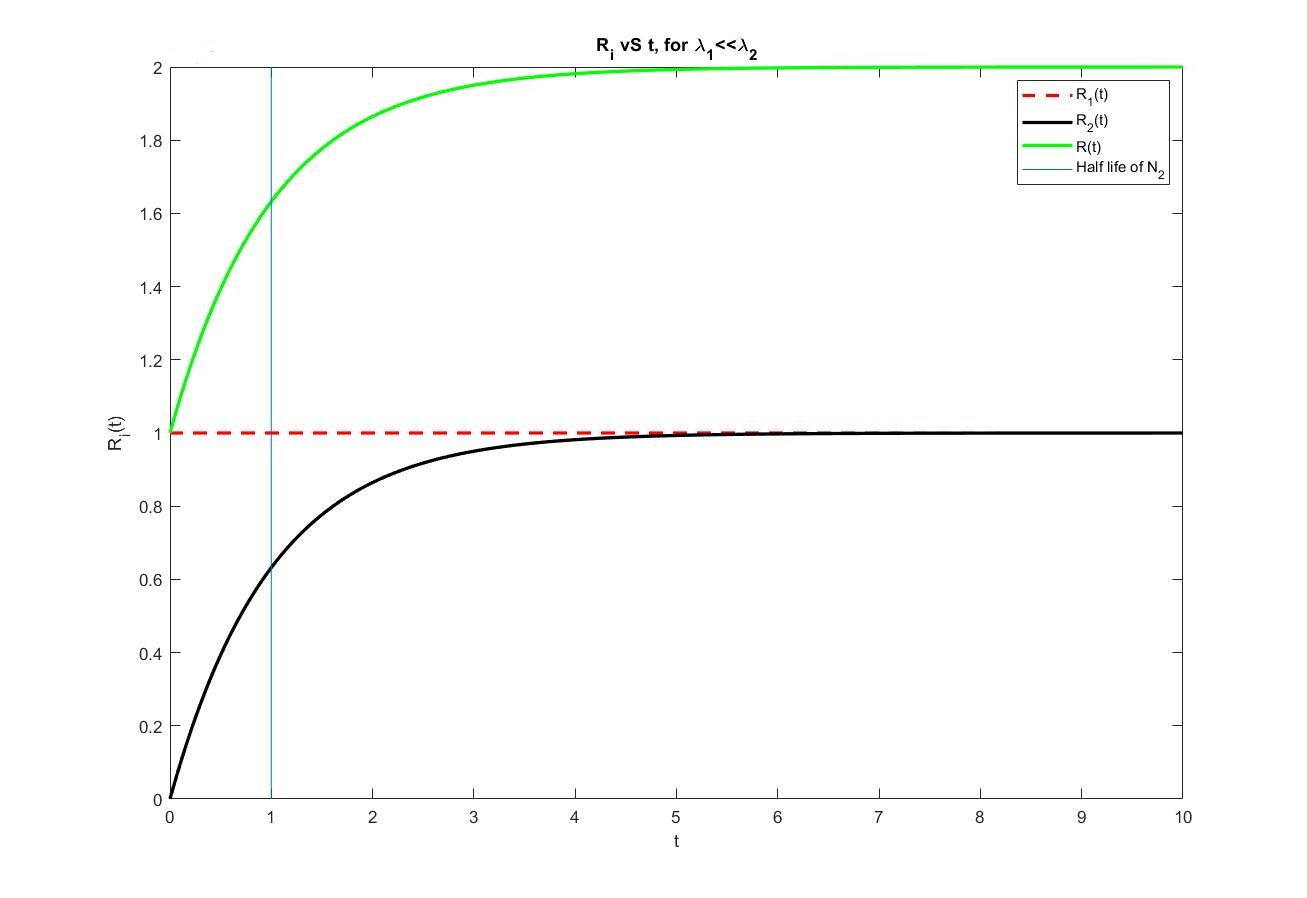
\includegraphics[scale=0.45]{R(t)}
		\caption{Γραφικές παραστάσεις για τις ενεργότητες όταν $\lambda_1<<\lambda_2$. \\
	$R(t) = R_1(t) + R_2(t)$}
		\label{fig2}
	\end{figure}
	
	Από τα παραπάνω συμπεραίνουμε πως για μεγάλο χρόνο από την δημιουργία της πηγής, οι δύο ενεργότητες για τους πυρήνες $^{90}Sr$ και $^{90}Υ$ θα έρθουν σε πυρηνική ισορροπία ακόμη και σε λίγα πολλαπλάσια του χρόνου ημιζωής του γρήγορα διασπώμενου Υτρίου. Έτσι, θεωρώντας πως πλέον είμαστε σε πολύ μεγάλο χρόνο από την δημιουργία της πηγής, μπορούμε να πούμε πως η ενεργότητά της είναι διπλάσια αυτής που υπολογίστηκε πιό πάνω στην υποενότητα \textit{"Ιδιότητες της Πηγής $^{90}Sr$"}, δηλαδή 
	\begin{align*}
			R_{correct} =&  2\cdot R \Rightarrow \\
						=& 1.26R_0\Rightarrow\\
				   \simeq& 2.8\times 10^4 \text{διασπάσεις/min}
	\end{align*}
	
	Τότε, από την σχέση (\ref{eq5}) έχουμε αναμενόμενες διασπάσεις σε γωνία Ω=0.22
		\begin{align*}
			N_\Omega = \frac{R\Omega}{4\pi} =\frac{2.8\times10^5\cdot0.22}{4\pi} \simeq 4900
		\end{align*}
		
	Δεδομένου ότι είχαμε 2700 διασπάσεις, τώρα ο συντελεστής απόδοσης του GM προκύπτει φυσιολογικά μικρότερος της μονάδας
	\begin{align*}
		M =& \frac{N_{exper}}{N_\Omega} \Rightarrow\\
		M \simeq&55\% 
	\end{align*}
	\\
\subsection*{Συμπεράσματα}
	Εν τέλει βρήκαμε πως τα σωματίδια με ενέργεια 2.2MeV έχουν εμβέλεια (1055$\pm$182)mg/cm$^2$ εντός των υλικών. Έτσι, για να βρούμε το πάχους του υλικού που θα μπορούσε να τα σταματήσει θα έπρεπε απλά να διαιρέσουμε με την πυκνότητά του.
	Ακόμη, είδαμε πως σε ενέργειες έως και 2.2MeV, η συνεισφορά της απώλειας ενέργειας των ηλεκτρονίων μέσω ακτινοβόλησης φωτονίων γ, είναι πολύ μικρότερη από την απώλεια μέσω διεγέρσεων/ιονισμών του υλικού μέσω της καμπύλης Bethe-Bloch.
	Τέλος, είδαμε πως αν αμελήσουμε την πυρηνική ισορροπία, θα έχουμε παράδοξα αποτελέσματα.
	
	
\end{document}